Test results for real agents were performed for agent devices forced to use half of their CPU capabilities and 512Mb of memory. Algorithms were grouped into a non-collaborative group (A*, Cloud A*) and a collaborative group (CA*, Cloud CA*). Results can be seen in Figures \ref{fig:on_prem_test_time} and in logarithmic scale on Figure \ref{fig:on_prem_test_time_log}. The vertical axis represents the sum of paths computing time in milliseconds and the vertical axis indicates the dimension of the map f.e map with dimension 5 will have 25 (5x5) possible locations for the agent.

\begin{figure}[H]
    \centering
    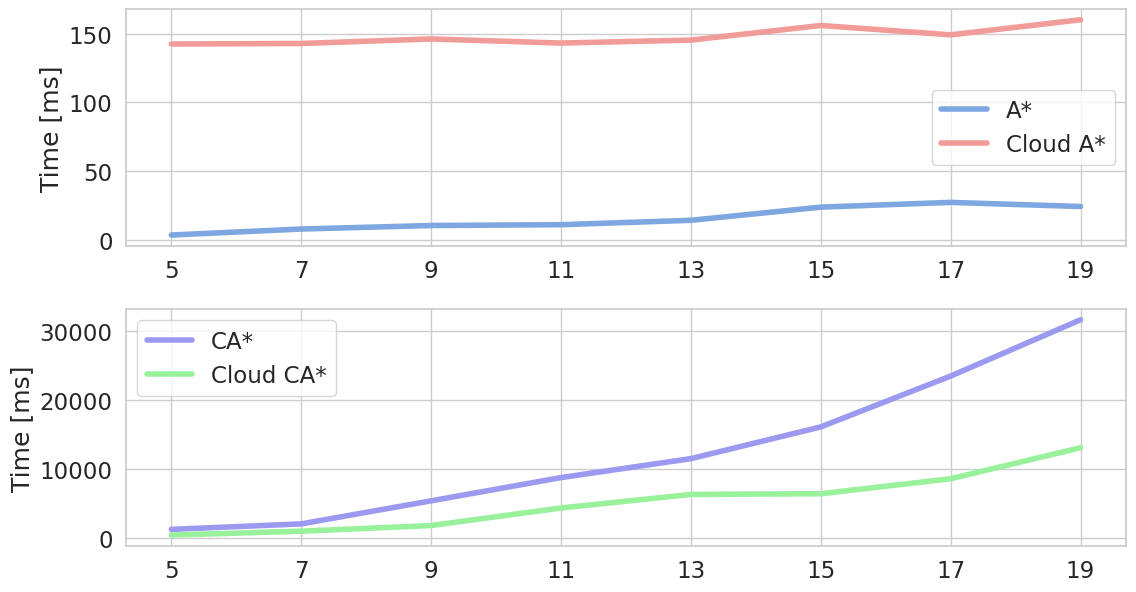
\includegraphics[width=0.75\textwidth]{pictures/on_prem_test_time.png}
    \caption{Test on on-prem setup}
    \label{fig:on_prem_test_time}
\end{figure}
\begin{figure}[H]
    \centering
    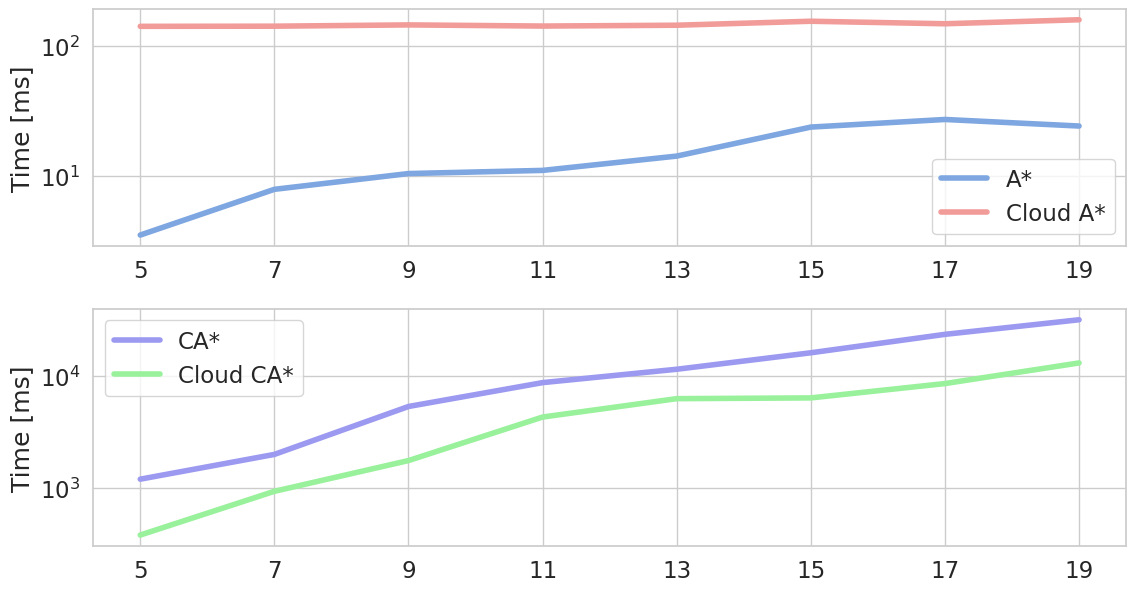
\includegraphics[width=0.75\textwidth]{pictures/on_prem_test_time_log.png}
    \caption{Test on on-prem setup in log scale}
    \label{fig:on_prem_test_time_log}
\end{figure}

The results of the performance testing indicate that non-collaborative algorithms are significantly faster than collaborative ones. The average time difference between A* and Cloud A* was found to be around 150 ms, with A* being faster. Additionally, the results show that Cloud A* has a higher deviation than A*.

When comparing the results of CA* and Cloud CA*, it was found that CA* outperforms Cloud CA* on the smallest map. However, on larger maps, Cloud CA* performed better. The average performance of Cloud CA* was found to be around 10 times faster than CA*.